\label{chapter:discussion}

In this part ParsBert V3 is used as pre-trained Bert model. PyTorch version is used. Due to hardware limitation train batch size is set to 4 and evaluation batch size is set to 8.
Model save into reports directory every 500 iteration. In first experiments whole data is used to fine-tune BERT model. As a result BERT is fine-tuned on news data set. Next step is to extract on layer before last one as embedding(a representation for each word) and replace task 4 embedding part with this model. 
Tokenization result for one sample is represented is Figure \ref{fig:fine}.

\begin{figure}
	\centering
	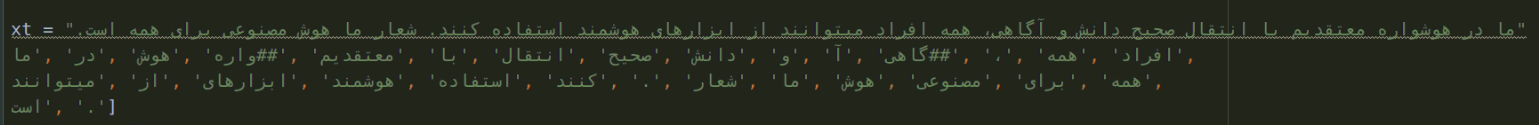
\includegraphics[width=15cm]{images/tkn.png}
	\caption{Tokenization based on BERT model for an input sentences.}
	\label{fig:fine}
\end{figure}